\documentclass{article}
\usepackage{graphicx}
\usepackage{amsmath}
\DeclareMathOperator{\sgn}{sgn}
\begin{document}

\begin{figure}[ht!]
\centering
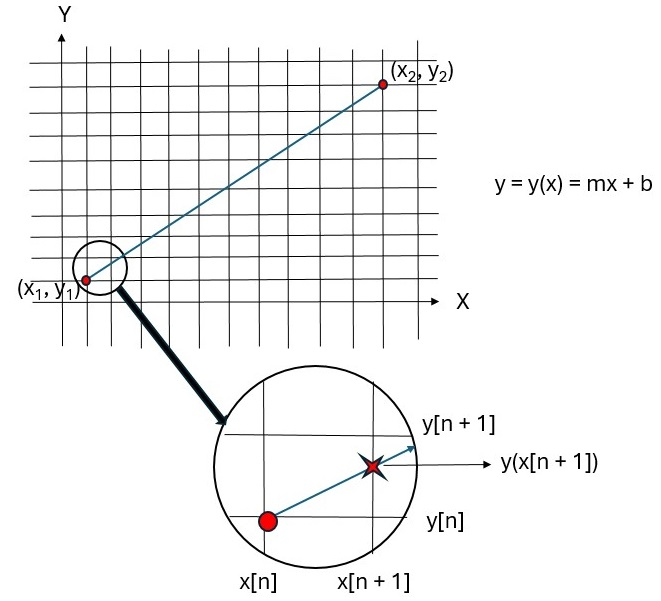
\includegraphics[width=90mm]{Line Rasterization.jpg}
\caption{Line Rasterization Algorithm \label{overflow}}
\end{figure}

\begin{enumerate}
    \item \text{Set Initial and Final values}
           \begin{align*}
                x[0] = x_{1}, x[N] = x_{2} \\ \\
                y[0] = y_{1}, y[N] = y_{2} \\ \\ 
             \end{align*}
    \item \text{\underline{for $n = 0 \rightarrow N - 2$:}} 
           \begin{align*}
                &x[n + 1] = x[n] + 1 \\ \\ 
                &y[n + 1] = \begin{cases}
                                y[n] \quad \quad \quad \quad \quad, \quad y\big(x[n + 1]\big) - y[n] < 0.5 \\ \\
                                y[n] + \sgn\big(\Delta y\big), \quad y\big(x[n + 1]\big) - y[n] \geq 0.5 
                              \end{cases} 
            \end{align*}
\end{enumerate}

\end{document}
